% !TEX root = ../apuntefinitos.tex
% !TEX encoding = UTF-8 Unicode
% !TeX spellcheck = es_ES

\chapter{Elementos 3D}
Para elementos tridimensionales se van a tener tres desplazamientos por nodo $u,v,w$. La matriz constitutiva para sólidos 3D se calcula según \eqref{eq:constitutive3D}

\begin{equation} \label{eq:constitutive3D}
\ME =\left[\begin{array}{cccccc} 2\,G+\lambda  & \lambda  & \lambda  & 0 & 0 & 0\\ \lambda  & 2\,G+\lambda  & \lambda  & 0 & 0 & 0\\ \lambda  & \lambda  & 2\,G+\lambda  & 0 & 0 & 0\\ 0 & 0 & 0 & G & 0 & 0\\ 0 & 0 & 0 & 0 & G & 0\\ 0 & 0 & 0 & 0 & 0 & G \end{array}\right] \qquad \ME^{-1}=\frac{1}{E}\left[\begin{array}{cccccc} 1 & -\nu  & -\nu  & 0 & 0 & 0\\ -\nu  & 1 & -\nu  & 0 & 0 & 0\\ -\nu  & -\nu  & 1 & 0 & 0 & 0\\ 0 & 0 & 0 & f & 0 & 0\\ 0 & 0 & 0 & 0 & f & 0\\ 0 & 0 & 0 & 0 & 0 & f \end{array}\right]
\end{equation}
donde 
\[
\lambda = \frac{E \nu}{(1+\nu)(1-2\nu)}, \qquad  G=\frac{E}{2(1+\nu)}, \qquad f = 2+2\nu
\]

Un esquema general para calcular la matriz de rigidez de un sistema compuesto por elementos 3D es el siguiente. Tenga en cuenta que falta la obtención de los puntos Gauss.
\begin{lstlisting}[caption={Programa generalizado para obtener \( \MK \) para elementos 3D.},numbers=left,label={cod:obtencion3Drigidez}]
%% Dofinitions
Ndofpornod = 3; Ndn = Ndofpornod;
n2d = @(n) repmat(n*Ndn,Ndn,1) - (Ndn-1:-1:0)'; % forma generalizada
[Nnod, Ndim] = size(nodos);
[Nelem, Nnodporelem] = size(elementos);
Ndofporelem  =  Ndofpornod*Nnodporelem;
dof = Ndofpornod*Nnod;
DOF = reshape(1:dof,Ndofpornod,[])';
%% Integracion
K = sparse(dof,dof);
for e = 1:Nelem
    ke = zeros(Ndofporelem,Ndofporelem);
    meindof = reshape(DOF(elementos(e,:),:)',1,[]);
    elenod = nodos(elementos(e,:),:);
    for ipg = 1:pg.n
        r = pg.u(ipg,1); s = pg.u(ipg,2); t = pg.u(ipg,3);
        Ns = eval(N);
        dNs = eval(dN); 
        jac = dNs*elenod;
        Djac = det(jac)/factor; % Ver tabla `\ref{tab:FactorJacobianoElemento}` `\label{line:jacFactor}`
        dNxyz = jac\dNs;
        B=zeros(size(E,2),Ndofpornod * Nnodporelem);
        B(1,1:3:end-2) = dNxyz(1,:); %dx
        B(2,2:3:end-1) = dNxyz(2,:); %dy  
        B(3,3:3:end)   = dNxyz(3,:); %dz VER PAGINA 80 Cook. Ec (3.1-9)
        B(4,1:3:end-2) = dNxyz(2,:); %dy
        B(4,2:3:end-1) = dNxyz(1,:); %dx
        B(5,2:3:end-1) = dNxyz(3,:); %dz
        B(5,3:3:end)   = dNxyz(2,:); %dy
        B(6,1:3:end-2) = dNxyz(3,:); %dz
        B(6,3:3:end)   = dNxyz(1,:); %dx
        ke = ke + B'*E*B*pg.w(ipg)*Djac;
    end
    K(meindof,meindof) = K(meindof,meindof) + ke;
end
\end{lstlisting}
donde la variable \texttt{factor} es aplicada según la geometría del elemento. Para elementos rectangulares o hexaedros el valor del factor es 1. 

\begin{table}[htb!]
    \centering
    \begin{tabular}{c|c}
        Elemento & Factor \\ \hline
        Triángulos & 2 \\
        Tetraedros & 6 \\
        Pirámides  &  3 \\
        \emph{Wedges}& 2  \\
    \end{tabular}
\caption{Factor que divide el determinante del jacobiano para varios elementos. Ver linea \ref{line:jacFactor} del código \ref{cod:obtencion3Drigidez}}
\label{tab:FactorJacobianoElemento}
\end{table}

\section{Formulación elemento hexaedro lineal (H8)}
El modelado con elementos isoparamétricos hexaedros de 8 nodos es un buen punto de partida para comenzar a manejar los elementos finitos en 3 dimensiones. Un código hecho para obtener $\MK$ con elementos H8 se adapta con facilidad para los H20.

\begin{figure}[htb!]
    \centering
    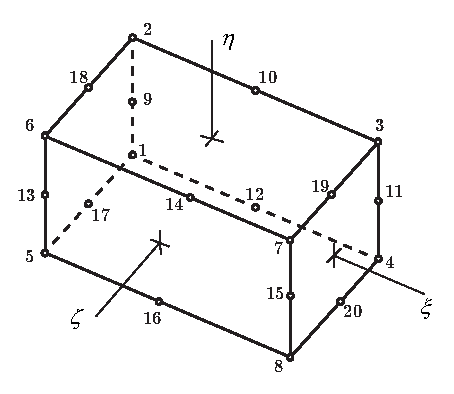
\includegraphics[width=.6\textwidth]{fig/H20numbering.eps}
    \caption{Numeración de nodos H20 en \Adina (Ejes sugeridos)}
    \label{fig:H20numbering}
\end{figure}

Cada nodo tendrá $3$ grados de libertad, dándonos $24$ \dof{} por elemento. El elemento H20 de la figura \ref{fig:H20numbering} esta planteado de tal forma que los primeros nodos del 1 al 8 son los nodos del H8 que se va formular a continuación.

La funcionalidad a usar es la siguiente

\[
X_{\mathrm{H8}} = \left[1, \xi, \eta, \zeta, \xi \eta, \xi \eta, \eta \zeta, \xi \eta \zeta \right]
\]



\subsubsection*{Formulación elementos}
El jacobiano tiene la forma
\[
\jac=
\left[\begin{array}{lll}\spartial{x}{\xi} & \spartial{y}{\xi}  & \spartial{z}{\xi}  \\ \spartial{x}{\eta}  &\spartial{y}{\eta}  &\spartial{z}{\eta} \\\spartial{x}{\zeta} & \spartial{y}{\zeta} &\spartial{z}{\zeta}\end{array}\right]
\]
pudiendo ser calculado de la siguiente forma

\begin{equation}
\jac = \begin{bmatrix}
\frac{\partial}{\partial \xi} \MN \\
\frac{\partial}{\partial \eta} \MN \\
\frac{\partial}{\partial \zeta} \MN 
\end{bmatrix}
\cdot 
\left[\begin{array}{lll}{x_{1}} & {y_{1}} & {z_{1}} \\ {x_{2}} & {y_{2}} & {z_{2}} \\ {x_{3}} & {y_{3}} & {z_{3}} \\ {x_{4}} & {y_{4}} & {z_{4}} \\ {x_{5}} & {y_{5}} & {z_{5}} \\ {x_{6}} & {y_{6}} & {z_{6}} \\ {x_{7}} & {y_{7}} & {z_{7}} \\ {x_{8}} & {y_{8}} & {z_{8}}\end{array}\right]
\end{equation}
donde la primer matriz termina siendo $3\times8$ para un elemento H8. La segunda matriz son las posiciones \textit{globales} de los nodos del elemento. El jacobiano se puede entonces utilizar para calcular

\begin{equation}
\Mme{\partial N}=\left[\begin{array}{l} \frac{\partial}{\partial x}\MN  \\ \frac{\partial}{\partial y} \MN  \\ \frac{\partial}{\partial z} \MN  \end{array}\right]=\jac^{-1}\left[\begin{array}{l}\frac{\partial}{\partial \xi} \MN \\
\frac{\partial}{\partial \eta} \MN \\ 
\frac{\partial}{\partial \zeta} \MN \end{array}\right]
\end{equation}
con lo obtenido se puede calcular la matriz $\MB$.

La matriz \textit{strain-deformation} queda
\[
\MB = \begin{bmatrix}
B_1 &B_2 &B_3 &B_4 &B_5 &B_6 &B_7 &B_8
\end{bmatrix}
\]
donde
\begin{equation}
B_{i}=\left[\begin{array}{ccc}{\partial N_{i} / \partial x} & {0} & {0} \\ {0} & {\partial N_{i} / \partial y} & {0} \\ {0} & {0} & {\partial N_{i} / \partial z} \\ {0} & {\partial N_{i} / \partial z} & {\partial N_{i} / \partial y} \\ {\partial N_{i} / \partial z} & {0} & {\partial N_{i} / \partial x} \\ {\partial N_{i} / \partial y} & {\partial N_{i} / \partial x} & {0}\end{array}\right]
\end{equation}

Finalmente un calcula la rigidez del elemento usando \eqref{eq:RigidezElemento}. Usando 8 puntos gauss se podría efectuar una integración \textit{full} del elemento. Usando la función \ref{cod:gauss}:
\begin{lstlisting}
pg = gauss([2 2 2]); % 8 pg para H8 
\end{lstlisting}

\section{Elemento tetraedro lineal (T4)}
Se espera que el lector ya haya programado elementos 2D y que tenga experiencia obteniendo las funciones de formas de elementos diversos. Esto dicho, el salto de elementos 2D a elementos 3D puede presentar dificultades debido a la falta de bibliografía acerca del tema, o la omisión de la aplicación de teoría por parte de los autores.

A continuación se dejan rutinas de \Matlab~ para que el usuario pueda rápidamente empezar a experimentar con tetraedros lineales. Se empieza procesando una malla de tetraedros cuadráticos de diez nodos para que se pueda resolver con un programa para tetraedros de cuatro nodos.

\lstinputlisting[caption = {Descarga y procesado de malla T10 para uso con rutinas para elementos T4.},label={cod:gauss}]{code/t4/t4dominio.m}

El próximo paso es definir el material en la matriz $\ME$ según la ecuación \eqref{eq:constitutive3D}. Antes de integrar usando la rutina \ref{cod:obtencion3Drigidez} se tienen que obtener las funciones de forma (Código \ref{cod:t4shapefun}) y definir la integración numérica según la tabla \ref{tab:gausstetraedros}

\lstinputlisting[caption = {Obtención de las funciones de forma para elementos T4.},label={cod:t4shapefun}]{code/t4/t4shapefun.m}


\begin{table}[htb!]
	\centering
	\begin{tabular}{cccc}
		Nro. Puntos & Orden & Coordenadas & Pesos \\ \hline \hline
		1 & 0 & \( \left(\frac{1}{4}, \,\frac{1}{4}, \, \frac{1}{4} \right)\) & 1 \\ [1pt] \hline
		4 & 1 & \(  (a,b,b), (b,b,b), (b,b,a), (b,a,b) \) & \( \frac{1}{4}\) \\ [2pt]
		&   &donde    \( a = \frac{5+3\sqrt{5}}{20}, \quad b =\frac{5-3\sqrt{5}}{20} \) & \\[2pt] \hline 
		5 & 2 & \( \left(\frac{1}{4}, \frac{1}{4}, \frac{1}{4} \right)\) & \( -\frac{4}{5}\)   \\[5pt]
		&   &  \( \left(\one{2},\one{6}, \one{6} \right), \left(\one{6},\one{6}, \one{6} \right), \left(\one{6},\one{6}, \one{2} \right), \left(\one{6},\one{2}, \one{6} \right) \) & \(\frac{9}{20}\)
	\end{tabular}
	\caption{Valores para la integración numérica de tetraedros usando cuadratura de Gauss.}
	\label{tab:gausstetraedros}
\end{table}

\begin{figure}[htb!]
	\centering
	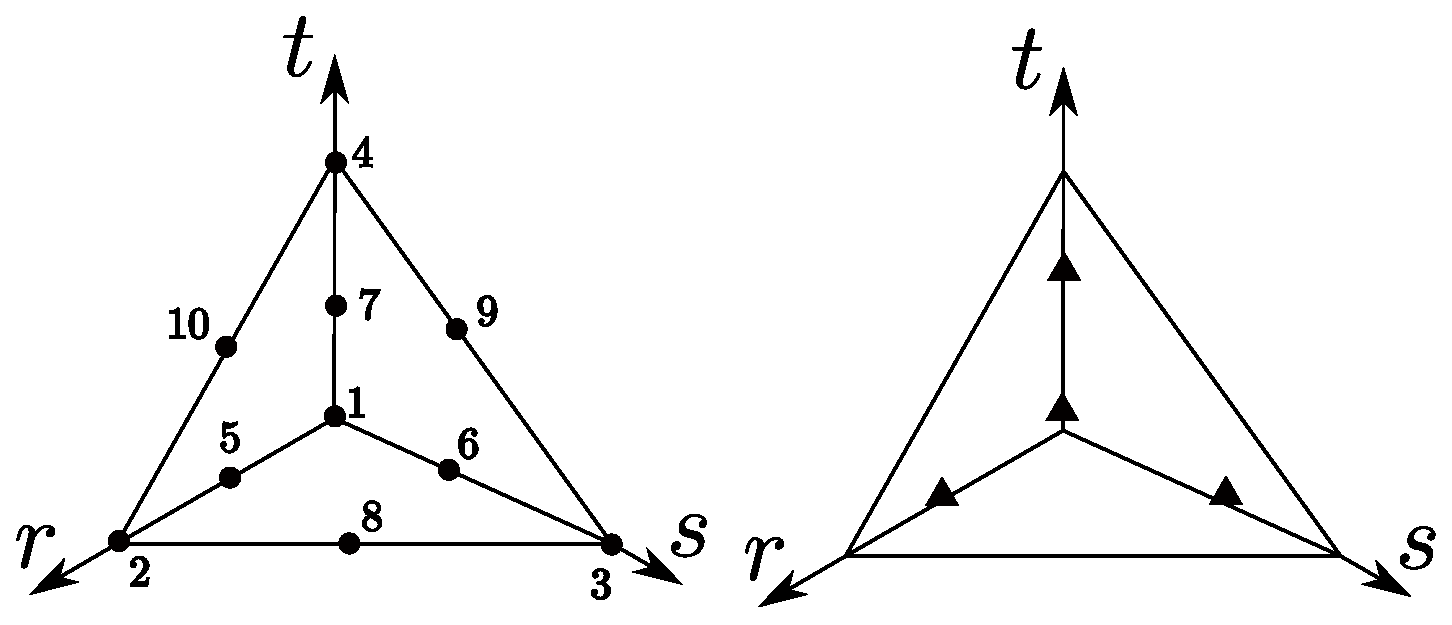
\includegraphics[width=0.8\textwidth]{fig/T10numbering.eps}
	\caption{Numeración de un tetraedro de diez nodos y la ubicación de los puntos Gauss para un grado de precisión 2 (orden 1).}
	\label{fig:T10numbering}
\end{figure}


%\lstinputlisting[caption = {gauss.m},label={cod:gauss}]{code/gauss.m}




